\documentclass[11pt]{article}
\usepackage{geometry}                
\geometry{letterpaper}                   

\usepackage{graphicx}
\usepackage{amssymb}
\usepackage{epstopdf}
\usepackage[square]{natbib}
\usepackage{amssymb, amsmath}
\usepackage{float}

\DeclareGraphicsRule{.tif}{png}{.png}{`convert #1 `dirname #1`/`basename #1 .tif`.png}

%\title{Self-Organized Criticality}
%\author{Nishant Dogra, Michael Wild}
%\date{date} 

\begin{document}




\thispagestyle{empty}

\begin{center}
\includegraphics[width=5cm]{ETHlogo.eps}

\bigskip


\bigskip


\bigskip


\LARGE{ 	Lecture with Computer Exercises:\\ }
\LARGE{ Modelling and Simulating Social Systems with MATLAB\\}

\bigskip

\bigskip

\small{Project Report}\\

\bigskip

\bigskip

\bigskip

\bigskip


\begin{tabular}{|c|}
\hline
\\
\textbf{\LARGE{Self-Organized Criticality and Phase Transitions }}\\
\textbf{\LARGE{in a Forest Fire Model}}\\
\\
\hline
\end{tabular}
\bigskip

\bigskip

\bigskip

\LARGE{Nishant Dogra, Michael Wild}



\bigskip

\bigskip

\bigskip

\bigskip

\bigskip

\bigskip

\bigskip

\bigskip

Zurich\\
December 2012\\

\end{center}



\newpage

%%%%%%%%%%%%%%%%%%%%%%%%%%%%%%%%%%%%%%%%%%%%%%%%%

\newpage
\section*{Agreement for free-download}
\bigskip


\bigskip


\large We hereby agree to make our source code for this project freely available for download from the web pages of the SOMS chair. Furthermore, we assure that all source code is written by ourselves and is not violating any copyright restrictions.

\begin{center}

\bigskip




\bigskip


\begin{tabular}{@{}p{3.3cm}@{}p{6cm}@{}@{}p{6cm}@{}}
\begin{minipage}{3cm}

\end{minipage}
&
\begin{minipage}{6cm}
\vspace{2mm} \large Name 1

 \vspace{\baselineskip}

\end{minipage}
&
\begin{minipage}{6cm}

\large Name 2

\end{minipage}
\end{tabular}


\end{center}
\newpage

%%%%%%%%%%%%%%%%%%%%%%%%%%%%%%%%%%%%%%%



% IMPORTANT
% you MUST include the ETH declaration of originality here; it is available for download on the course website or at http://www.ethz.ch/faculty/exams/plagiarism/index_EN; it can be printed as pdf and should be filled out in handwriting


%%%%%%%%%% Table of content %%%%%%%%%%%%%%%%%

\tableofcontents

\newpage

%%%%%%%%%%%%%%%%%%%%%%%%%%%%%%%%%%%%%%%



\section{Abstract}

\section{Individual contributions}

\section{Introduction and Motivations}
\subsection{What is Self-Organized Criticality?}
Self-Organized Criticality is the Concept that the dynamics of a physical system converge to a critical point independant of the bestowed boundary conditions. This critical point commonly is not the equilibrium point in a traditional, physical sense. The concept is best understood by example, so we shall bring up a very educative one introduced first by \cite{bak88} ). 
Imagine a sand pile in 2 dimensions. One can discretisze this pile into cells, which are denoted with the indices $n$. Each of those cells has an amount of sand grains on it, which is directly corresponding to the height $z_{n}$. Now we state the simple rule, that, if the difference in height between two neighboring cells becomes larger than a predefined limit, the higher cell will give grains to the lower cell (avalanche). Now every timestep, we drop a grain on cell one. Independant of the initial conditions, eventually, a straight slope will evolve. The critical point is reached if every difference between two neighboring cells is exactly the limit. What happens if we drop the next grain? Then the difference $z_{1}-z_{2}>p$ and one grain will drop on $z_{2}$. Subsequently, the difference $z_{2}-z_{3}$ will be too big and the process repeats until it hits the last cell. We therefore call a state critical if a yet so small disturbance can propagate throughout the whole system. A further condition for SOC is the presence of the critical point, in the example, that would be the slope that should form in every experiment independant of the starting conditions. 
It is important to note here, that this critical state is \emph{not} the equilibrium state of the system, since that would be a flat surface. 

\subsection{What is Self-Organized Criticality}
Self-organized criticality (SOC) is a concept applied to spacially extended dynamic physical systems. It is often quite difficult to descripe the temporal and spatial evolution of such a system and a lot of research happens in that field. Usually, one uses a mean-field approach to such a problem, where the indidual coupled degrees of freedom are replaced by a field. This (external) field then acts on the DOF.  SOC is a different approach to this problem. It is the concept, that a certain class of dissipative, coupled dynamic systems converge to a critical point independantly of their underlying boundary and initial conditions. 
What are the properties of such a critical point? First of all, it is stable with respect to small disturbances. If this was not true, the system would not evolve to such a point. Note that this does not imply that such a point \emph{exists}. If a certain point is unstable, the system commonly will not evolve to this point. The critical point, however, generally is not the physical equilibrium point of the system.

\subsection{Flicker Noise}
Flicker noise is something often mentioned when talking about dissipative coupled dynamical systems. Flicker Noise (or $1/f$-Noise) is the description for an often observed phenomenon of such systems; The observation, that the power spectrum $S(f)$ scales with $1/f$ or more generally, with $f^{-\beta}$. This implies that $S(f)\cdot f \varpropto 1$

\subsection{Forest-Fire Model}
A Forest Fire Model is basically a cellular automata. Each cell has three possible states:
\begin{enumerate}
\item Empty Site
\item Alive Tree
\item Burning Tree
\end{enumerate}
There are four rules defined for each cell, which are executed simultaneously:
\begin {itemize}
\item A burning tree turns into an empty site
\item A tree starts to burn if at least one of its neighbors are burning
\item A tree will grow on an empty site randomly with probability $p$
\item A tree will burn randomly with probability $f$

\end{itemize}
It is important to note that the Forest Fire Model does not only apply to forest fires as its name would suggest. A whole class of problems follows the same basic rules and can be treated accordingly. An example would be the spreading of a disease, where one can directly transform the above rules and states.

\subsection{Power Laws}
Power laws are functions of the form $ P(s) \varpropto s^{-\tau}$ . These functions are found in many data sets, such as the size distribution of cities in a certain area. Take any country, one will find one very large metropolis, a few large cities, many medium sized towns and a huge lot of small towns. Power laws imply that the frequency of a general data point is inversely proportional to its magnitude. 

In context to the FFM, it is proposed as a way of quantifying the frequency of Fires with respect to their cluster size. 

Power laws have also prominently been found in data sets of earthquakes, where they apply almost perfectly, meaning that small earthquakes happen very often in respect to the frequency of big ones.

\subsection{Key Parameters in SOC}

To find out wether a basic FFM exhibits SOC behavior, we need to define a set of parameters which serves as indicators for the desired analysis. 
\begin{itemize}

\item The time needed to burn down a forest cluster: This is heavily dependant on the form of the implementation. If we choose to implement it in a way like [reference needed], we will have an instantaneous fire which essentially takes no time to burn and just resets all the connected trees. If however, we choose the form of a “visible” fire, meaning that the ratio $f/p\ll1$  is not 0  in limit and that it takes the fire one timestep to advance a grid cell, then the time needed to burn a forest cluster is an important variable we need to extract from the simulation.

\item Number distribution of the size of clusters: Here we first need to define what a cluster is. A cluster is a set of neighboring cells all obtaining the same state. When we talk about forest clusters, we of course mean connected trees. In the implementation where the fire spreads infinitly fast, the forest cluster containing the ignitor cell is the same as the burnt area. The size distribution therefore is a very good indicator for the fire size distribution. 

\item The mean number of forest clusters in a unit volume $n(s)$ , where s  is the number of trees in a cluster. 

\item Number of fires per unit time step: This is a tuning parameter of the model.

\item Correlation length.
\end{itemize}
We have tried to implement the model in a way that the measurment of these desired variables is possible with the least needed effort.

\subsection{Motivation}
Why is it important to study these effects? As mentioned before, forest fire models apply to a wide range of problems and are therefore helpful in predicting the behaviour of such systems. Self-Organized criticality is the concept that describes the dynamics of such models and the two fields are therefore closely connected. One has closely studied these effects to make better predictions about forest fires. The main problem was, that in most cases, even relatively small fires were extinguished by the authorities. Since that led to an overcritical state, the probability for a huge, devastating fire rose quickly. This has happended in the past and had a serios impact on the ecosystem of those areas.
Since the problem of self-organized criticality has been understood, one has stopped to extinguish every little fire, therefore avoiding to reach an overcritical state at which the disturbance (a small fire) can propagate throughout the whole system (large-scale fire). 
The same ideas can be applied to a variety of problems such as disease spreading or urban planning.


\section{Description of the Model}
\subsection{Cellular automata}

A cellular automata is a very powerful way of simulating problems which are defined by a set of rules. It is usually simulated on a grid, but not necessarily restricted to those geometrical constraints. The main characteristics are:
\begin{itemize}
\item Every grid point has a state

\item Grid points change their state depending on the neighbor states according to a set of rules

\item Random actions may be introduced
\end{itemize}

In the example of the FFM, every grid point has three states (empty, alive and burning) and four rules, the most obvious of which is “change state to burning if you are alive and your neighbor is burning”. 

Cellular Automata can exhibit very complicated behavior when fed with very simple rules, which is the main reason why they are so powerful. There are similarities to agent-based models and networks, but it is not to be mistaken for one of these.


The second approach to grid-based updating is with a second grid that stores temporary information. [Insert Description here]


\section{Implementation}
As discussed before, there are two main implementation methods for the model: One way is to update the whole grid every timestep, whereas the second method picks a cell randomly at every timestep an only updates the chosen one.
Both versions store the Grid in a Matrix which is initialized as follows:
\begin{verbatim}
Grid=zeros(Grid_Size);
\end{verbatim}
or if the grid should be filled by a degree of $k$:
\begin{verbatim}
Grid=floor(rand(Grid_Size)+k);
\end{verbatim}
\subsection{Grid Based Updating}
The basic construct of the grid based updating implementation looks like this:
\begin{verbatim}
for i=1:t % Loop over all timesteps
    for j=1:size(Grid,1) % Loop over all y-coordinates
        for k=1:size(Grid,2) % Loop over all x-coordinates
            if Grid(j,k)==0 %If the grid point is empty
                //Grid(j,k)=1 with some probability p
            end
        end
    end
    for j=1:size(Grid,1) % Loop over all y-coordinates
        for k=1:size(Grid,2) % Loop over all x-coordinates
            //if Neighbor(j,k)==3 % If grid neighbor is burning
                Grid(j,k)=2 % Set current grid point on fire
            end
        end
    end
    for j=1:size(Grid,1) % Loop over all y-coordinates
        for k=1:size(Grid,2) % Loop over all x-coordinates
            if Grid(j,k)==3 % If Grid point is burning
                Grid(j,k)=0; % Turn it into an empty site
            end
            if Grid(j,k)==2 % If grid point is ignited
                Grid(j,k)=3; % Turn it into an empty site.
            end
        end
    end
end
\end{verbatim}
Several things are to note here:
\begin{itemize}
\item Commands with // in front are not implemented exactly like that. Check the appendix for the complete source code.
\item We need several spatial loops in order to successfully suppress updating fragments like infinite fire propagation speed in updating direction. 
\item For the same reason, we need a differention between newly ignited (state 2) and burning (state 3) trees. 
\item The Algorithm is quite slow because of all the loops and if-statements.
\end{itemize}


\subsection{Random Based Updating}
In a random based updating implementation, at the beginning of every time step, one random cell is chosen. It then checks for the rules of the model and acts accordingly. In order to see fires, we need to have instantaneous burning, which is actually permitted by the model. However, it changes the dynamics of the system drastically. But more about that later. The following steps are taken for each timestep:

\begin{enumerate}
\item Choose a single cell
\item If cell is empty, grow a tree with probability $p$
\item If cell is a tree, with probabiltiy $f$, burn it and the connected cluster
\end{enumerate}
In Matlab, this looks something like this:
\begin{verbatim}
for i=1:t % Loop over all timesteps
(j,k)=ceil(Grid_Size*rand(1,2)); % Choose a random cell
	if  Grid(j,k)==0 % If the cell is empty
		\\With some probability p set G(j,k)==1;
	end
	if Grid(j,k)==1 % If the cell is alive
		\\with some probability f execute burn(j,k);
	end
end
\end{verbatim}

This implementation of the forest fire model has several advantages:
\begin{itemize}
\item There are no problems due to updating processes
\item Much shorter implementation
\item Easier to extract data
\end{itemize}
The last point is to be explained more extensively: Every time a tree ignites, the whole connected cluster is burned down. Since the whole process happens in a single timestep, there are no big issues.

\subsubsection{keeping track of the clusters}
Keeping track of the different clusters was more difficult than we thought at first, but we managed to find an elegant solution. It works by keeping a second grid which stores all the cluster indices. This has several advantages:
\begin{itemize}
\item if a new tree grows, we can just look at the neighbor cluster index to determine the current cell index
\item if a tree burns, we simply delete all the trees with the same index as the burned tree.
\end {itemize}
 \paragraph * {Problems and Solutions}
Problems arose quickly. Here is a short summary of all the major problems and the corresponding solutions:
\subparagraph {Storing the indices}
The problem here was to find a way to store all possible cluster indices and their availability. Since the maximum number of clusters can be easily found to be $Nc_{max}= \frac{G^2}{2}$  (imagine a perfect chessboard-layout filling half of the grid; if one more is added, they combine into a bigger cluster), we already knew the size of the vector. The final format was a Matrix with $Nc_{max}$ Columns and 2 rows. The first row would simply store all the possible indices from 1 to $Nc_{max}$ and the second row would store the corresponding binary information about the availability.
\subparagraph{growing a tree between two clusters}
It is simple to determine the cluster index of a new tree if there is just one neighbor. The big problem arises if there are more than two neighbors with \emph{different} cluster indices. The solution to this problem was that we set the index as the lower of both neighbors and changed the whole cluster with the higher index to the lower one. This was relatively easy to do by using the matlab built-in function |ismember| which searches for all entries with a certain value and returns a matrix containing only that information. 

\subsection{The \emph{neighbor} function}
The \emph{neighbor} function is the same for both implementations. It takes the current cell coordinates  $(j,k)$ and returns a vector containing the coordinates of its direct neighbors. It works like this:
\begin{verbatim}
Set all neighbors to standard
// Ex: West_X=j-1; West_Y=k;
Treat Special cases
// Ex: if j==1
// West_X=size(Grid,1);
\end{verbatim}
Note that the \emph{neighbor} function creates periodic boundary conditions. 


\section{Simulation Results and Discussion}
\emph{note that in this section, $\Theta$ is defined as $p/f$.}
\subsection{Tree population}
A first step in the analysis of the results is to have a close look a the tree population during the simulation. Here are two examples:
\begin{figure}[H]
\centering
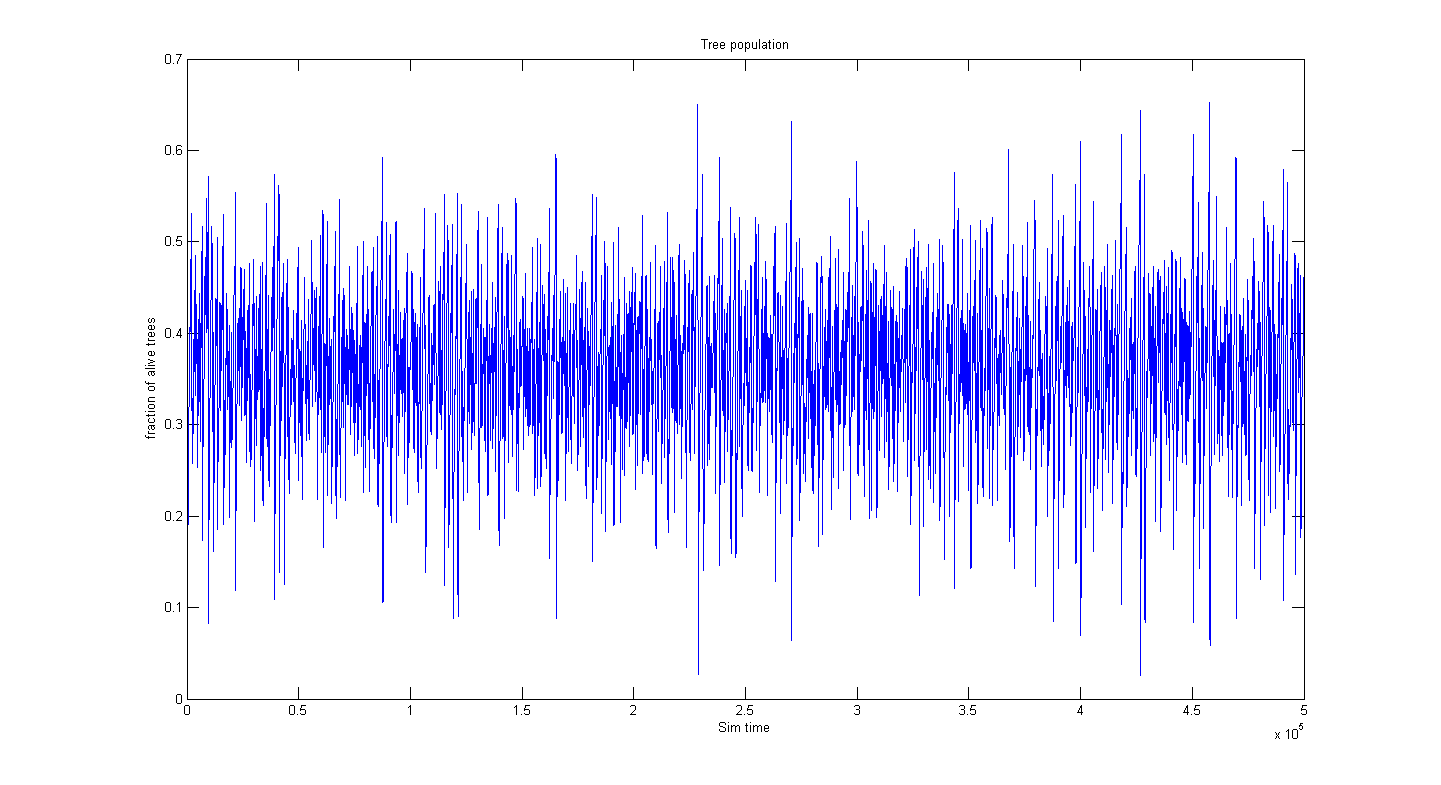
\includegraphics[width=0.9\textwidth,keepaspectratio=true,]{Pictures/Tree_Pop_50_1000_500000.png}
\caption{$N=50$, $\Theta=1000$, Simulation time 500'000}
\end{figure}
\begin{figure}[H]
\centering
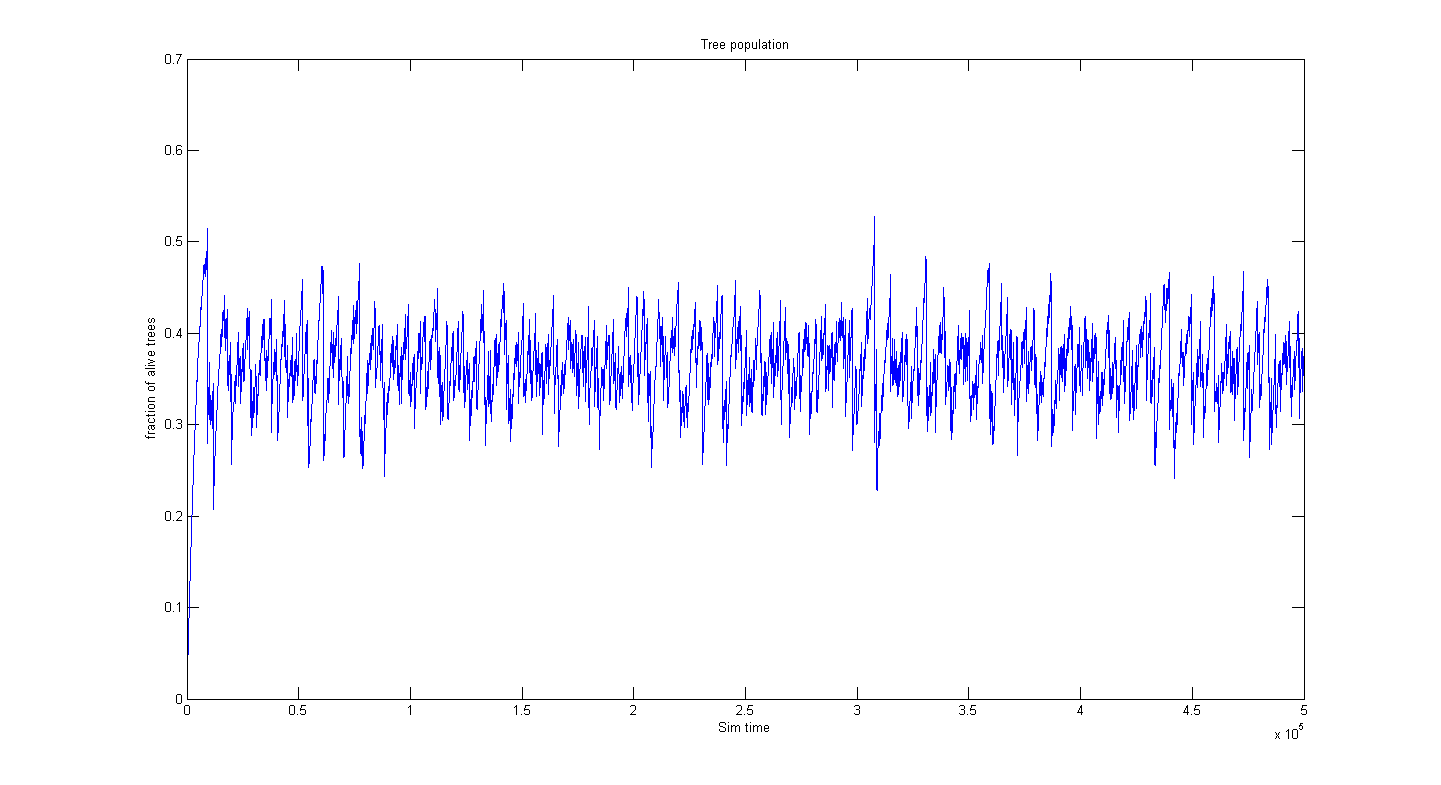
\includegraphics[width=0.9\textwidth,keepaspectratio=true,]{Pictures/Tree_Pop_100_100_500000.png}
\caption{$N=100$, $\Theta=100$, Simulation time 500'000}
\end{figure}
What can we learn from these plots? Well, in the first figure, Theta is equal to $10^3$, which is a moderatly large number. Yet, the plot of the tree fraction looks like random noise.We are not quite sure what we should interpret from such a plot. At $\Theta=100$, the plot looks a lot more stable, more like an actual \emph{equilibrium} point. Re-running the simulation with the same $\Theta$ but changed $f$ yields the same, consistent picture; after a short transient period to overcome the initial condition, the plot approximates a straight line. 
Now we know that the SOC state is not generally an equilibrium state and further insight into the properties of the system can only be achieved by analysis of other properties.
\subsection{Cluster Radius}
The Cluster Radius is defined as the root mean of all the distances of all cells of a cluster to their common center. This property should, given an SOC behaviour of the system, exhibit a power-law-behaviour that would be described as $S(r)=r^{-\beta}$ where$S(r)$ is the number of occurrences of clusters with radius r. In theory, what this means is, if you plot a double-logarithmic histogram of all cluster radii, it should give us a straight line with slope $\beta$. Of course, we expected a little "noise", given that our simulation was not infinite in time and space, but it should have approached it pretty well. Here is one of those double-logarithmic histograms:
\begin{figure}[H]
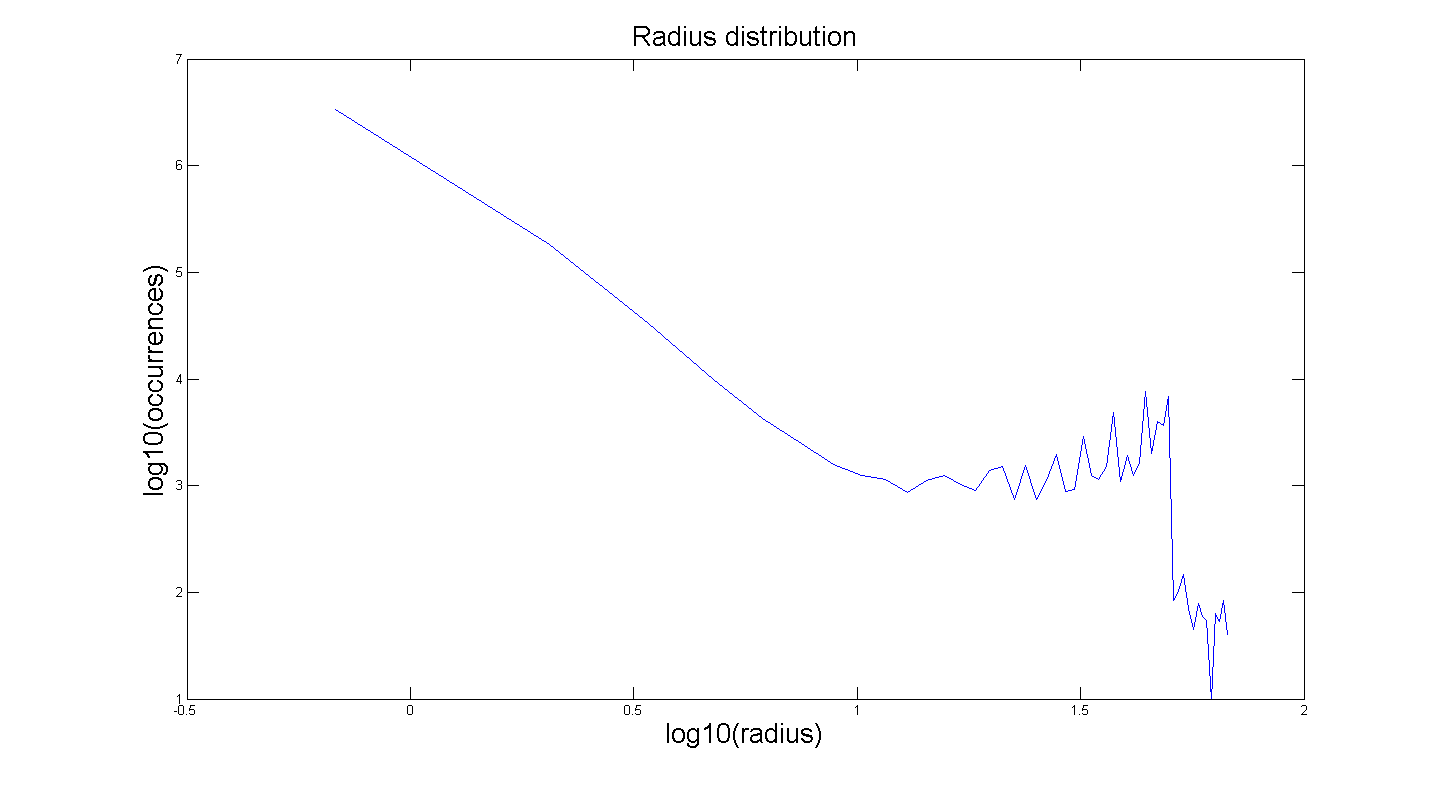
\includegraphics[width=0.9\textwidth,keepaspectratio=true]{Pictures/Radius_dist_1.png}
\caption{Cluster radius distribution ($N=100$, $\Theta=1000$, Sim Time 500'000)}
\end{figure}
\paragraph*{The Problem} that we see here is one that's closely related to the periodic boundary conditions. Imagine an empty grid with a small cluster that stretches from one side \emph{over the boundary} to the other side. Its center will be in the middle, but its radius will be much larger than it actually is. We guess that this causes the tilt that one can observe at medium sized clusters. We are currently working on a way to get around that problem. 


\subsection{Cluster Size}
The cluster size is another variable that we can easily measure. Here is a log-log-histogram of a simulation:
\begin{figure}[H]
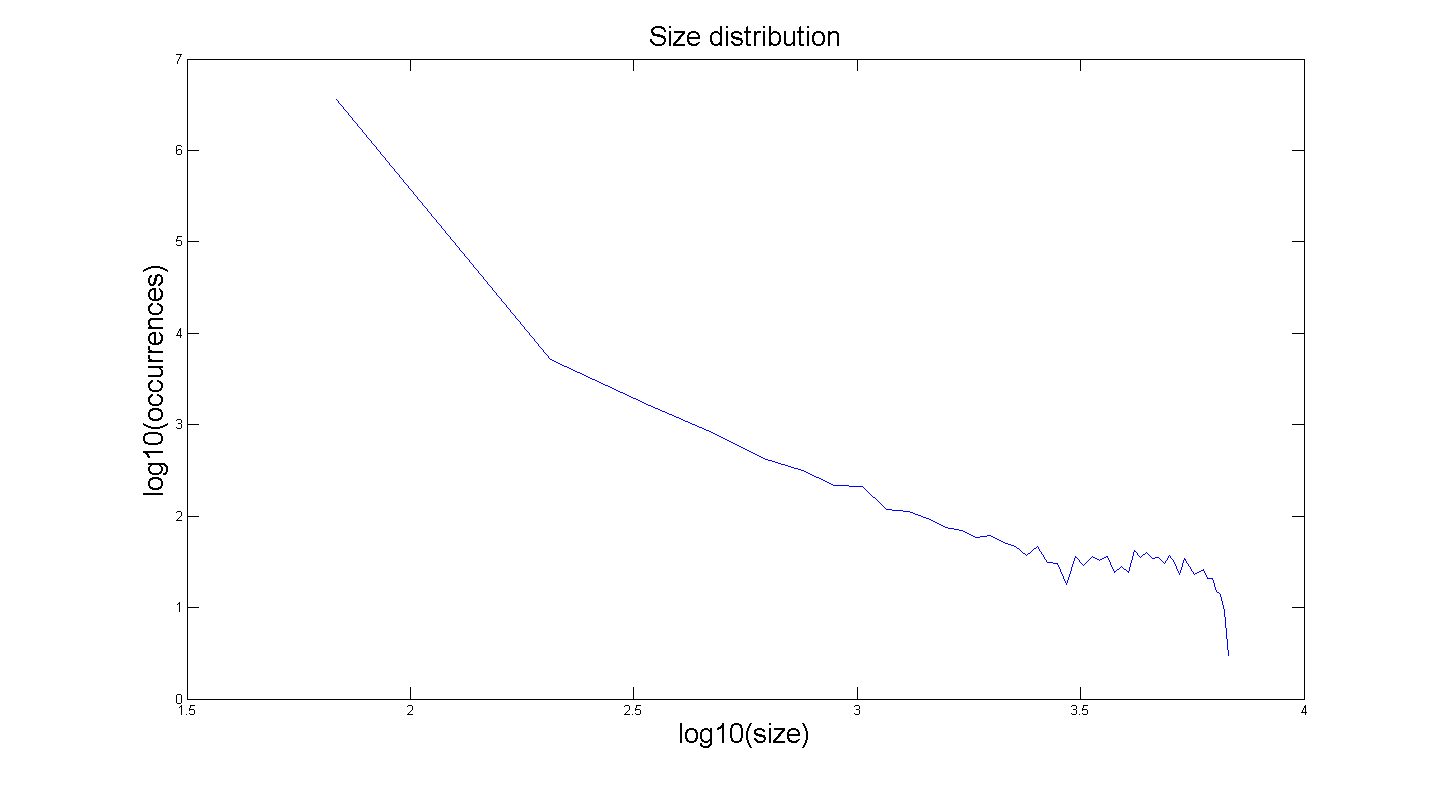
\includegraphics[width=0.9\textwidth,keepaspectratio=true]{Pictures/Size_dist_1.png}
\caption{Cluster size distribution ($N=100$, $\Theta= 1000 $, Sim Time 500'000  ) }
\end{figure}


\section{Open Questions}
We are wondering if it is "correct" to implement the forest fire in such a way with zero fire burning time like stated in \cite{pruessner04}. We have thus implemented two separate models, one of which uses finite burning speeds, while the other one (described in this text) uses infinite burning speed. Looking at the different timescales, it is obvious that the spreading of a fire should be very fast, but is it correct to use this in the limit of instantaneous fires?



\section{Summary and Outlook}

\begin{thebibliography}{9}
\bibitem{pruessner04}
	Gunnar Pruessner, Henrik Jeldtoft Jensen.
	\emph {A new, efficient algorithm for the Forest Fire Model},
	Phys. Rev. E 70 066707-1--25,
	2004
\bibitem{bak88}
	Per Bak, Chao Tang, Kurt Wiesenfeld.
	\emph{Self-organized criticality}
	Phys Rev. A 38 1,
	1988
\end{thebibliography}









\end{document}  



 
